\documentclass[10pt,aspectratio=169]{beamer}

% Theme and styling
\usetheme{Madrid}
\usecolortheme{default}
\setbeamertemplate{navigation symbols}{}
\setbeamertemplate{footline}[frame number]

% Packages
\usepackage{amsmath}
\usepackage{amssymb}
\usepackage{pifont}
\usepackage{xcolor}
\usepackage{tikz}
\usepackage{subcaption}
\usepackage{graphicx}
\usepackage{algorithm}
\usepackage{algorithmicx}
\usepackage{algpseudocode}
% \usepackage{enumitem}  % Conflicts with beamer
\usepackage{mathtools}
\usepackage{bm}

\definecolor{mygreen}{rgb}{0,0.6,0}
\definecolor{myred}{rgb}{0.8,0,0}
\newcommand{\greenoplus}{\textcolor{mygreen}{\ding{51}}}
\newcommand{\redominus}{\textcolor{myred}{\ding{55}}}

% Custom commands
\newcommand{\R}{\mathbb{R}}
\DeclareMathOperator{\atan}{atan2}

% Title information
\title{Scene Representation Paradigms for \\ Multimodal Trajectory Prediction}
\author{Your Name}
\institute{Computer Science Department}
\date{\today}

\begin{document}

% Title slide
\frame{\titlepage}

% Outline slide
\begin{frame}{Outline}
\tableofcontents
\end{frame}

\section{Introduction to Scene Representations}

\begin{frame}{Why Scene Representations Matter}
\begin{block}{Core Challenge}
How do we translate perception outputs into tensors that neural modules can effectively exploit for trajectory prediction?
\end{block}

\vspace{0.5cm}

\begin{columns}[T]
\column{0.6\textwidth}
\textbf{Desirable Properties:}
\begin{enumerate}
    \item High geometric fidelity
    \item Invariance to global transformations $SE(2) \rtimes \mathbb{R}$
    \item Information density
    \item Efficient spatio-temporal modeling
    \item Computational re-use across frames
\end{enumerate}

\column{0.35\textwidth}
\begin{alertblock}{Impact}
The choice of scene representation fundamentally affects the predictor's capacity to capture essential relationships and produce accurate motion forecasts.
\end{alertblock}
\end{columns}
\end{frame}

\section{Scene Representation Paradigms}

\begin{frame}{Two Main Paradigms}
\begin{figure}[H]
\centering
\begin{subfigure}[t]{0.35\textwidth}
    \centering
    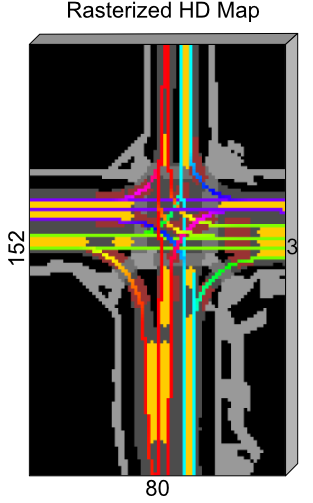
\includegraphics[width=\textwidth]{docs/latex/figures/caspnet-bev-repr.png}
    \caption{Rasterized BEV encoding}
    \label{fig:rasterized}
\end{subfigure}
\hfill
\begin{subfigure}[t]{0.37\textwidth}
    \centering
    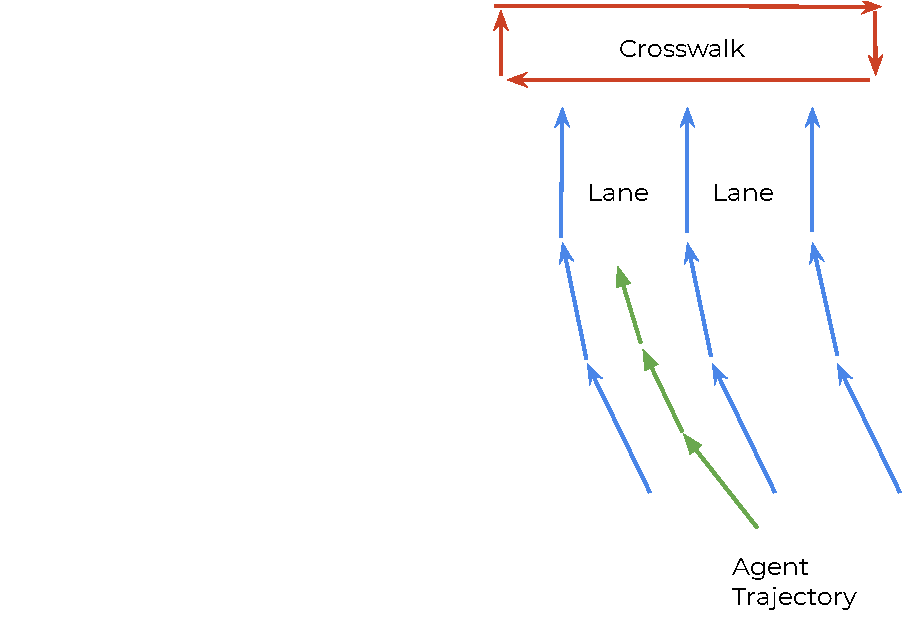
\includegraphics[width=\textwidth]{docs/latex/figures/vectornet-2020-vector-repr.pdf}
    \caption{Vectorized polyline preservation}
    \label{fig:vectorized}
\end{subfigure}
\end{figure}

\begin{itemize}
    \item \textbf{Rasterized}: Stack trajectories and HD maps into BEV images
    \item \textbf{Vectorized}: Preserve geometric polylines and relationships
\end{itemize}
\end{frame}

\subsection{Rasterized Approaches}

\begin{frame}{Raster Grid Representations}
\begin{columns}[T]
\column{0.6\textwidth}
\textbf{Key Components:}
\begin{itemize}
    \item BEV stack of past agent trajectories: $\mathbf{I}_d \in \mathbb{R}^{T_p \times H \times W \times F_d}$
    \item Static HD-map raster: $\mathbf{I}_s \in \mathbb{R}^{H \times W \times F_s}$
    \item Leverage convolutional backbones
    \item Runtime independent of number of agents
\end{itemize}

\textbf{Examples:} CASPNet family, MultiPath, TNT

\column{0.35\textwidth}
\begin{block}{Advantages}
\begin{itemize}
    \item Mature CNN architectures
    \item Scalable runtime
    \item Good spatial locality
\end{itemize}
\end{block}

\begin{alertblock}{Limitations}
\begin{itemize}
    \item Limited geometric fidelity
    \item Redundant pixel information
    \item Agent identity issues
    \item Shared coordinate system only
\end{itemize}
\end{alertblock}
\end{columns}
\end{frame}

\subsection{Vectorized Approaches}

\begin{frame}{Vector Representations}
\textbf{Core Principle:} Encode agents and lanes as vectorized geometric primitives

\vspace{0.3cm}

\begin{columns}[T]
\column{0.48\textwidth}
\textbf{Lane Representations:}
\begin{itemize}
    \item \textbf{Point-based}: $L_p^i = [P_1^i, P_2^i, \ldots, P_K^i]$
    \item \textbf{Segment-based}: $L_v^i = [V_1^i, V_2^i, \ldots, V_{K-1}^i]$ where $V_{k}^i = [P_k^i, P_{k+1}^i]$
\end{itemize}

\column{0.48\textwidth}
\textbf{Agent Trajectories:}
\begin{itemize}
    \item \textbf{Trajectory points}: $\mathcal{T}_{in}^a = [P_1^a, P_2^a, \ldots, P_T^a]$
    \item \textbf{Motion vectors}: $M_t^a = [P_{2}^a - P_{1}^a, \ldots, P_{T}^a - P_{T-1}^a]$
\end{itemize}
\end{columns}

\vspace{0.3cm}

\begin{block}{Key Benefits}
\begin{itemize}
    \item Higher geometric fidelity
    \item Explicit modeling of spatio-temporal relationships
    \item Enables graph/transformer architectures
    \item More compact representation
\end{itemize}
\end{block}
\end{frame}

\section{Query-Centric Paradigm}

\begin{frame}{Limitations of Agent-Centric Approaches}
\begin{columns}[T]
\column{0.65\textwidth}
\textbf{Agent-Centric Issues:}
\begin{itemize}
    \item Single global frame centered on ego vehicle
    \item Roto-translation invariance only for center agent
    \item Computationally infeasible for factorized attention
    \item Must re-encode entire scene at each timestep
\end{itemize}

\textbf{Factorized Attention Complexity:}
\begin{align}
\text{Temporal:} &\quad \mathcal{O}(N_{\max}T^{2}) \\
\text{Agent}\leftrightarrow\text{Map Fusion:} &\quad \mathcal{O}(N_{\max}T K) \\
\text{Agent}\leftrightarrow\text{Agent Fusion:} &\quad \mathcal{O}(N_{\max}^{2}T)
\end{align}

\column{0.3\textwidth}
\begin{alertblock}{Problem}
Cubic complexity in dense traffic scenarios leads to significant computational overhead.
\end{alertblock}
\end{columns}
\end{frame}

\begin{frame}{Query-Centric Solution}
\begin{figure}[ht]
\centering
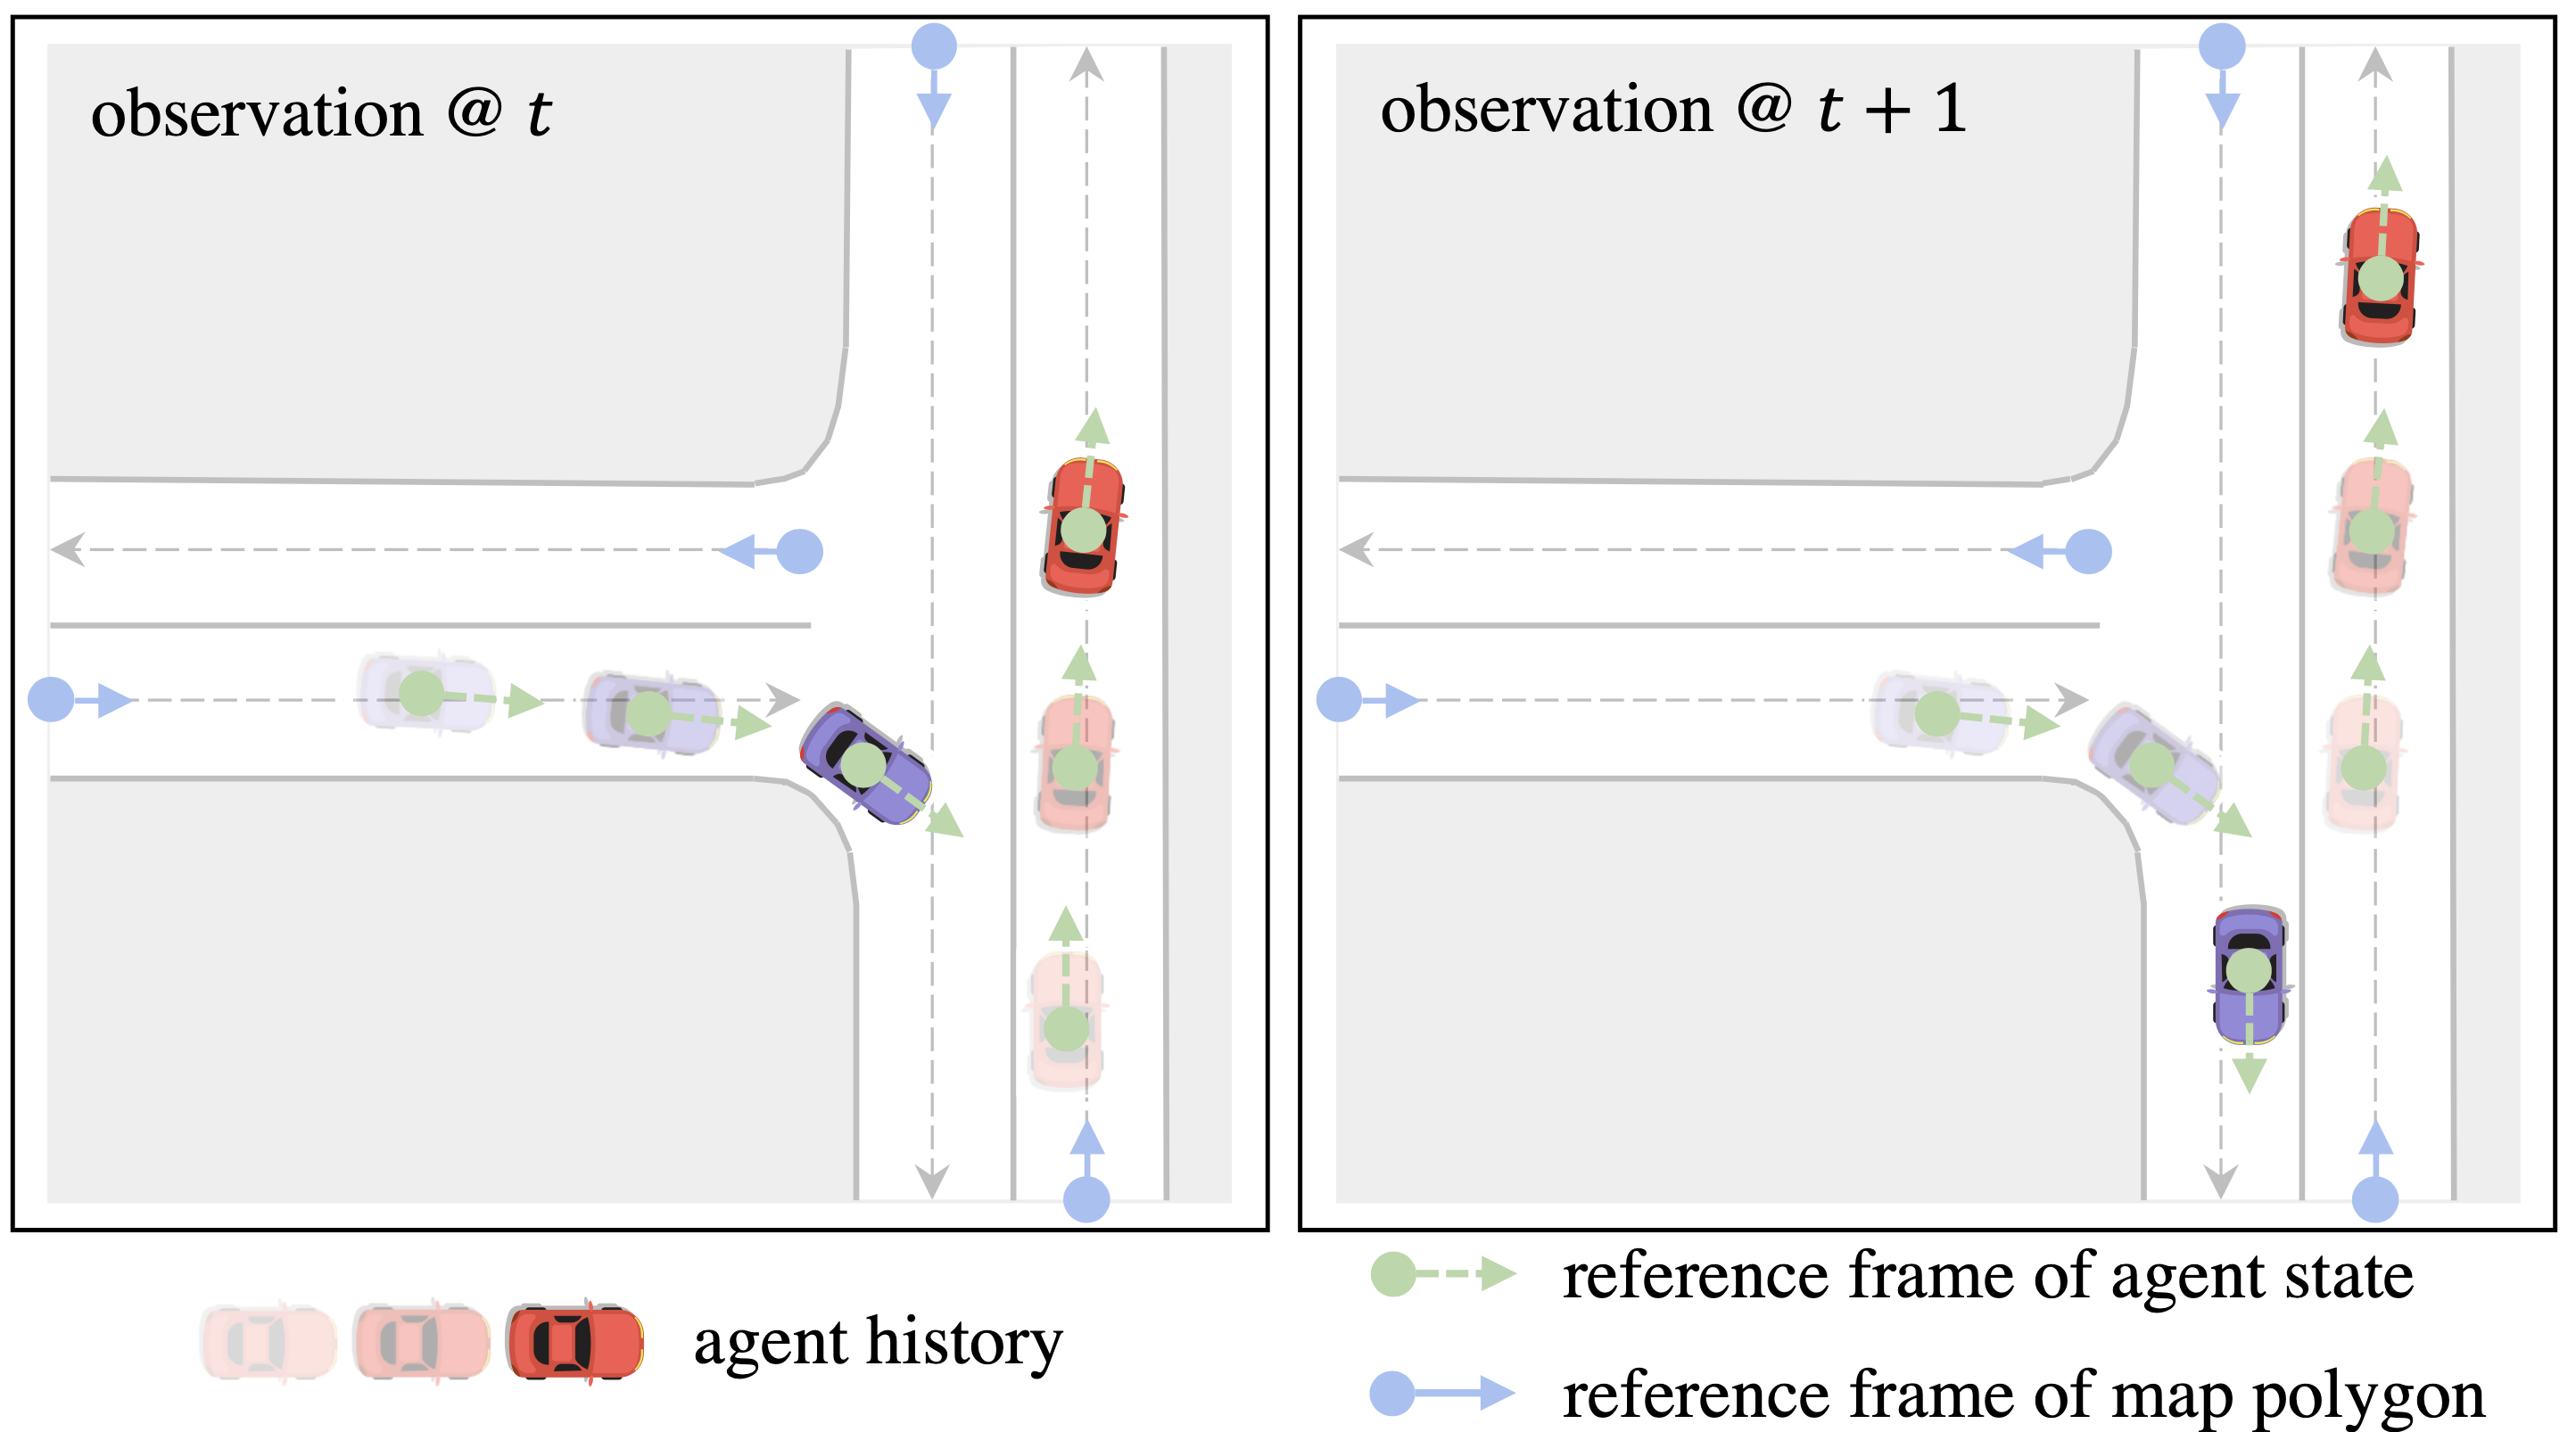
\includegraphics[width=0.6\textwidth]{docs/latex/figures/qc_reference_frame.png}
\caption{Each scene entity lives in its own local coordinate system}
\end{figure}

\textbf{Key Insight:} Establish a \emph{local coordinate system} (fiber) for each scene element

\begin{block}{Computational Benefits}
\begin{center}
\scriptsize
$\underbrace{\mathcal{O}(N_{\max}T^2)+\mathcal{O}(N_{\max}TL)+\mathcal{O}(N_{\max}^2T)}_{\text{agent-centric factorized attention}}
\longrightarrow
\underbrace{\mathcal{O}(N_{\max}T)+\mathcal{O}(N_{\max}L)+\mathcal{O}(N_{\max}^2)}_{\text{query-centric streaming}}$
\end{center}
\end{block}
\end{frame}

\subsection{Local Frame Construction}

\begin{frame}{Local Frame Construction}
\textbf{Agent States:} For the $i$-th agent at timestep $t$, local frame anchored at $\mathbf{p}_i^t = (p_{i,x}^t, p_{i,y}^t)$ with $x$-axis aligned to heading $\theta_i^t$:

\begin{equation}
\mathbf{x}^{(i,t)}_{\text{local}} = \mathbf{T}_{i,t}^{-1} \mathbf{x}_{\text{global}}^{(i,t)}, \quad
\mathbf{T}_{i,t} = \begin{bmatrix}
\cos\theta_i^t & -\sin\theta_i^t & p_{i,x}^t \\
\sin\theta_i^t & \cos\theta_i^t & p_{i,y}^t \\
0 & 0 & 1
\end{bmatrix} \in \mathrm{SE}(2)
\end{equation}

\vspace{0.3cm}

\textbf{Map Elements:} Each segment's start vertex acts as origin, first segment direction defines $x$-axis

\begin{block}{Result}
$N_{\max} \times T$ distinct fibers over observation window, each with standardized local representation
\end{block}
\end{frame}

\begin{frame}{Fiber Bundle Visualization}
\begin{figure}[ht]
\centering
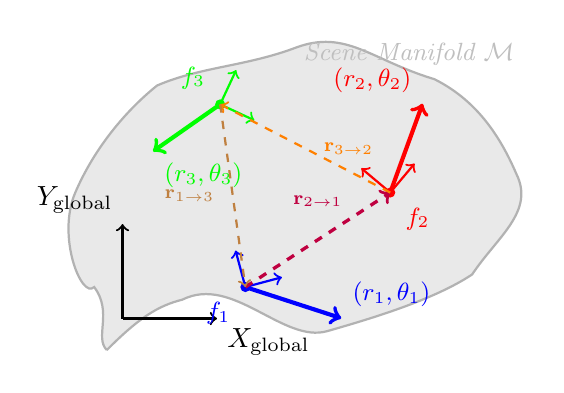
\begin{tikzpicture}[scale=0.8]
  % Complex 2D manifold
  \coordinate (origin) at (0,0);
  \coordinate (p1) at (1.2,0.8);
  \coordinate (p2) at (3.5,0.3);
  \coordinate (p3) at (5.8,1.2);
  \coordinate (p4) at (6.5,2.8);
  \coordinate (p5) at (5.2,4.3);
  \coordinate (p6) at (3.0,4.8);
  \coordinate (p7) at (0.8,4.2);
  \coordinate (p8) at (-0.5,2.5);
  \coordinate (p9) at (-0.2,1.0);

  % Manifold surface
  \fill [gray!25, opacity=0.7]
        (origin) ..
        controls (0.5,0.5) and (0.8,0.7) ..
        (p1) ..
        controls (2.0,1.2) and (2.8,0.1) ..
        (p2) ..
        controls (4.2,0.5) and (5.2,0.8) ..
        (p3) ..
        controls (6.2,1.8) and (6.8,2.2) ..
        (p4) ..
        controls (6.2,3.5) and (5.8,4.0) ..
        (p5) ..
        controls (4.2,4.6) and (3.8,5.1) ..
        (p6) ..
        controls (2.2,4.5) and (1.5,4.5) ..
        (p7) ..
        controls (0.3,3.8) and (-0.2,3.2) ..
        (p8) ..
        controls (-0.8,1.8) and (-0.4,0.8) ..
        (p9) ..
        controls (0.1,0.6) and (-0.2,0.2) ..
        (origin) -- cycle;

  % Manifold boundary
  \draw [gray!60, thick]
        (origin) ..
        controls (0.5,0.5) and (0.8,0.7) ..
        (p1) ..
        controls (2.0,1.2) and (2.8,0.1) ..
        (p2) ..
        controls (4.2,0.5) and (5.2,0.8) ..
        (p3) ..
        controls (6.2,1.8) and (6.8,2.2) ..
        (p4) ..
        controls (6.2,3.5) and (5.8,4.0) ..
        (p5) ..
        controls (4.2,4.6) and (3.8,5.1) ..
        (p6) ..
        controls (2.2,4.5) and (1.5,4.5) ..
        (p7) ..
        controls (0.3,3.8) and (-0.2,3.2) ..
        (p8) ..
        controls (-0.8,1.8) and (-0.4,0.8) ..
        (p9) ..
        controls (0.1,0.6) and (-0.2,0.2) ..
        (origin);

  \node[gray!50, font=\small\itshape] at (4.8,4.7) {Scene Manifold $\mathcal{M}$};

  % Global axes
  \draw[thick,->] (0.25,0.5) -- (1.75,0.5) node[anchor=north west]{$X_{\text{global}}$};
  \draw[thick,->] (0.25,0.5) -- (0.25,2) node[anchor=south east]{$Y_{\text{global}}$};

  % Fiber positions
  \coordinate (e1) at (2.2,1.0);
  \coordinate (e2) at (4.5,2.5);
  \coordinate (e3) at (1.8,3.9);

  % Fiber origins
  \draw[blue,fill=blue]   (e1) circle(2pt) node[below left=2pt] {\small$f_1$};
  \draw[red,fill=red]     (e2) circle(2pt) node[below right=2pt] {\small$f_2$};
  \draw[green,fill=green] (e3) circle(2pt) node[above left=2pt] {\small$f_3$};

  % Local reference frames
  \draw[blue,thick,->]   (e1) -- ++(15:0.6)  node[anchor=south west] {};
  \draw[blue,thick,->]   (e1) -- ++(105:0.6) node[anchor=south east] {};

  \draw[red,thick,->]    (e2) -- ++(50:0.6)  node[anchor=south west] {};
  \draw[red,thick,->]    (e2) -- ++(140:0.6) node[anchor=south east] {};

  \draw[green,thick,->]  (e3) -- ++(-25:0.6) node[anchor=north west] {};
  \draw[green,thick,->]  (e3) -- ++(65:0.6)  node[anchor=south west] {};

  % Motion vectors in local coordinates
  \draw[blue,->,line width=1.5pt]   (e1) -- ++( -18:1.6) node[anchor=south west] {\small$(r_1,\theta_1)$};
  \draw[red,->,line width=1.5pt]    (e2) -- ++(70:1.5) node[anchor=south east] {\small$(r_2,\theta_2)$};
  \draw[green,->,line width=1.5pt]  (e3) -- ++(-145:1.3) node[anchor=north west] {\small$(r_3,\theta_3)$};

  % Relative descriptors
  \draw[purple,dashed,->,very thick] (e1) -- (e2)
    node[midway,above=8pt,align=center] {\scriptsize$\mathbf{r}_{2\to 1}$};
  \draw[orange,dashed,->,thick] (e2) -- (e3)
    node[midway,right=3pt] {\scriptsize$\mathbf{r}_{3\to 2}$};
  \draw[brown,dashed,->,thick]  (e3) -- (e1)
    node[midway,left=3pt] {\scriptsize$\mathbf{r}_{1\to 3}$};
\end{tikzpicture}
\caption{Query-centric representation as fiber bundle with local coordinates and relative descriptors}
\end{figure}
\end{frame}

\subsection{Relative Descriptors}

\begin{frame}{Relative Descriptors and Embeddings}
For any pair of scene elements with tuples $(\mathbf{p}_i^t, \theta_i^t, t)$ and $(\mathbf{p}_j^s, \theta_j^s, s)$:

\begin{equation}
\mathbf{r}_{j\to i}^{s\to t} = \left[
    \|\mathbf{p}_j^s-\mathbf{p}_i^t\|_2,\;
    \atan(p_{j,y}^s-p_{i,y}^t, p_{j,x}^s-p_{i,x}^t)-\theta_i^t,\;
    \theta_j^s-\theta_i^t,\;
    s-t
\right]
\end{equation}

\vspace{0.5cm}

\textbf{4D Descriptor Components:}    \begin{enumerate}
    \item \textbf{Distance:} $\|p_j^s-p_i^t\|_2$ - spatial separation
    \item \textbf{Bearing:} $\atan(\cdot)-\theta_i^t$ - relative direction in local frame
    \item \textbf{Orientation:} $\theta_j^s-\theta_i^t$ - relative heading
    \item \textbf{Time:} $s-t$ - temporal offset
\end{enumerate}

\begin{block}{Key Property}
Invariant under global $SE(2)$ transformations, lifted to high-frequency representation via Fourier features
\end{block}
\end{frame}

\subsection{Geometric Perspective}

\begin{frame}{Fundamental Symmetries}
Query-centric paradigm exploits three key symmetries:

\vspace{0.3cm}

\begin{description}
\item[\textbf{Permutation Invariance}]
Agents form unordered sets—no element privileged. For permutation $\sigma$: $f(\sigma \cdot S) = \rho(\sigma) f(S)$

\item[\textbf{SE(2) Invariance}]
Rigid transformations leave encoding unchanged:
\begin{equation}
f_{\boldsymbol{\Psi}}(g \cdot S) = f_{\boldsymbol{\Psi}}(S) \quad \forall g \in SE(2)
\end{equation}

\item[\textbf{Temporal Translation Invariance}]
Sliding time windows: $f(S(t+\tau)) = f(S(t))$ for any $\tau \in \mathbb{R}$
\end{description}

\begin{block}{Geometric Insight}
    % Geometric Insight: Breaks intractable global manifold into small, repeatable sub-manifolds
Global scene manifold factorizes into isomorphic fibers—each representing standardized spatial/kinematic variables connected by simple relations
\end{block}
\end{frame}

\begin{frame}{Fiber Bundle Decomposition}
\begin{columns}[T]
\column{0.6\textwidth}
\textbf{Key Hypothesis:}
\begin{itemize}
    \item Model splits capacity between learning:
    \begin{enumerate}
        \item Relations between fibers
        \item Simple structures within fibers
    \end{enumerate}
    \item Avoids learning non-decomposable global manifold
    \item Pairwise encodings inhabit simpler manifold
\end{itemize}

\textbf{Inductive Bias:}
\begin{itemize}
    \item Respects symmetries
    \item Breaks intractable global manifold into small, repeatable sub-manifolds
    \item More data-efficient and interpretable
\end{itemize}

\column{0.35\textwidth}
\begin{block}{Benefits}
\begin{itemize}
    \item Reduced hypothesis space
    \item Better generalization
    \item Computational efficiency through streaming
    \item Natural multi-agent handling
\end{itemize}
\end{block}

\begin{alertblock}{Trade-off}
Query-centric models trade \textbf{compute} for \textbf{memory}
\end{alertblock}
\end{columns}
\end{frame}

\subsection{Comparison and Conclusions}

\begin{frame}{Memory Considerations}
\begin{columns}[T]
\column{0.6\textwidth}
\textbf{Query-Centric Memory Cost:}
\begin{itemize}
    \item Every agent state and map segment owns persistent token for each timestep
    \item All pairwise keys/values cached for streaming
    \item Scene tensor grows linearly with $N_{\max}T$
    \item Can reach hundreds of MB per batch
\end{itemize}

\textbf{QCNet Example:}
\begin{itemize}
    \item Single model training: $\sim 160$ GB GPU VRAM
    \item Typically requires 8x RTX 3090 (24GB)
    \item 10s sliding window with 128 agents: >10 GB
\end{itemize}

\column{0.35\textwidth}
\begin{block}{Mitigation Strategies}
\begin{itemize}
    \item Cache raw descriptors, not embeddings
    \item Compute embeddings on-the-fly
    \item Sparse attention mechanisms
    \item Deformable attention
\end{itemize}
\end{block}

\begin{alertblock}{Conclusion}
High memory cost stems from architecture complexity and caching, not the paradigm itself
\end{alertblock}
\end{columns}
\end{frame}

\begin{frame}{Paradigm Comparison}
\begin{table}[ht]
\centering
\footnotesize
\begin{tabular}{|p{2.5cm}|p{4cm}|p{4cm}|}
\hline
\textbf{Aspect} & \textbf{Rasterized} & \textbf{Query-Centric} \\
\hline
\textbf{Representation} & BEV image grids & Local coordinate frames \\
\hline
\textbf{Geometric Fidelity} & Limited by discretization & High, preserves relationships \\
\hline
\textbf{Computational Complexity} & $\mathcal{O}(H \times W)$ & $\mathcal{O}(N_{\max}^2)$ streaming \\
\hline
\textbf{Memory Usage} & Moderate & High (caching) \\
\hline
\textbf{Invariances} & Partial & Full SE(2) × $\mathbb{R}$ invariance \\
\hline
\textbf{Multi-agent} & Challenging & Natural \\
\hline
\textbf{Streaming} & Re-encode entire scene & Efficient caching \\
\hline
\textbf{Architecture} & CNN-based & Transformer/Graph-based \\
\hline
\end{tabular}
\end{table}

\begin{block}{Key Takeaway}
Query-centric paradigm offers superior theoretical properties and streaming efficiency at the cost of increased memory requirements
\end{block}
\end{frame}

\begin{frame}{Summary}
\begin{columns}[T]
\column{0.5\textwidth}
\textbf{Key Contributions:}
\begin{itemize}
    \item Fundamental symmetries in trajectory prediction
    \item Fiber bundle geometric perspective
    \item Computational efficiency through streaming
    \item Natural multi-agent capabilities
\end{itemize}

\textbf{Applications:}
\begin{itemize}
    \item QCNet, QCNeXt
    \item LMFormer
    \item Modern trajectory prediction models
\end{itemize}

\column{0.45\textwidth}
\begin{block}{Future Directions}
\begin{itemize}
    \item Memory optimization techniques
    \item Sparse attention mechanisms
    \item Hybrid approaches
    \item Real-time deployment
\end{itemize}
\end{block}

\begin{alertblock}{Impact}
Query-centric paradigm represents a fundamental shift towards more principled, efficient, and scalable trajectory prediction
\end{alertblock}
\end{columns}
\end{frame}


%==============================================================================
% LMFormer Section
%==============================================================================
\section{Review of Selected Architectures}

\subsection{LMFormer: A Query-Centric Approach}

\begin{frame}{LMFormer: A Query-Centric Approach}
    \begin{figure}
        \centering
        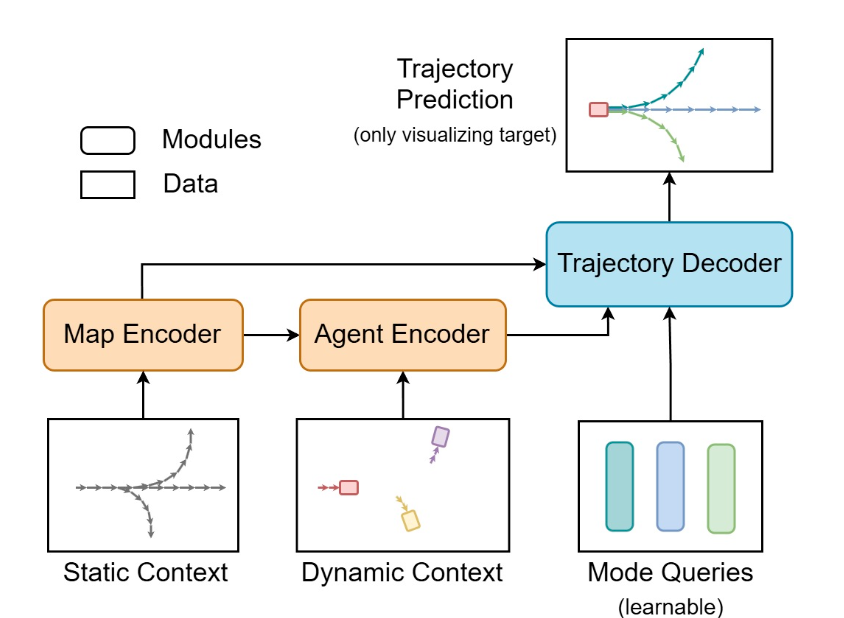
\includegraphics[width=0.9\textwidth]{docs/figures/lmformer_arch.png}
        \caption{LMFormer architecture: transformer encoders for static and dynamic contexts \& recurrent cross-attention decoder with coarse-to-fine refinement~\cite{lmformerYadav2025}.}
    \end{figure}
\end{frame}

\begin{frame}{LMFormer: Encoder Architecture}
    \begin{figure}
        \centering
        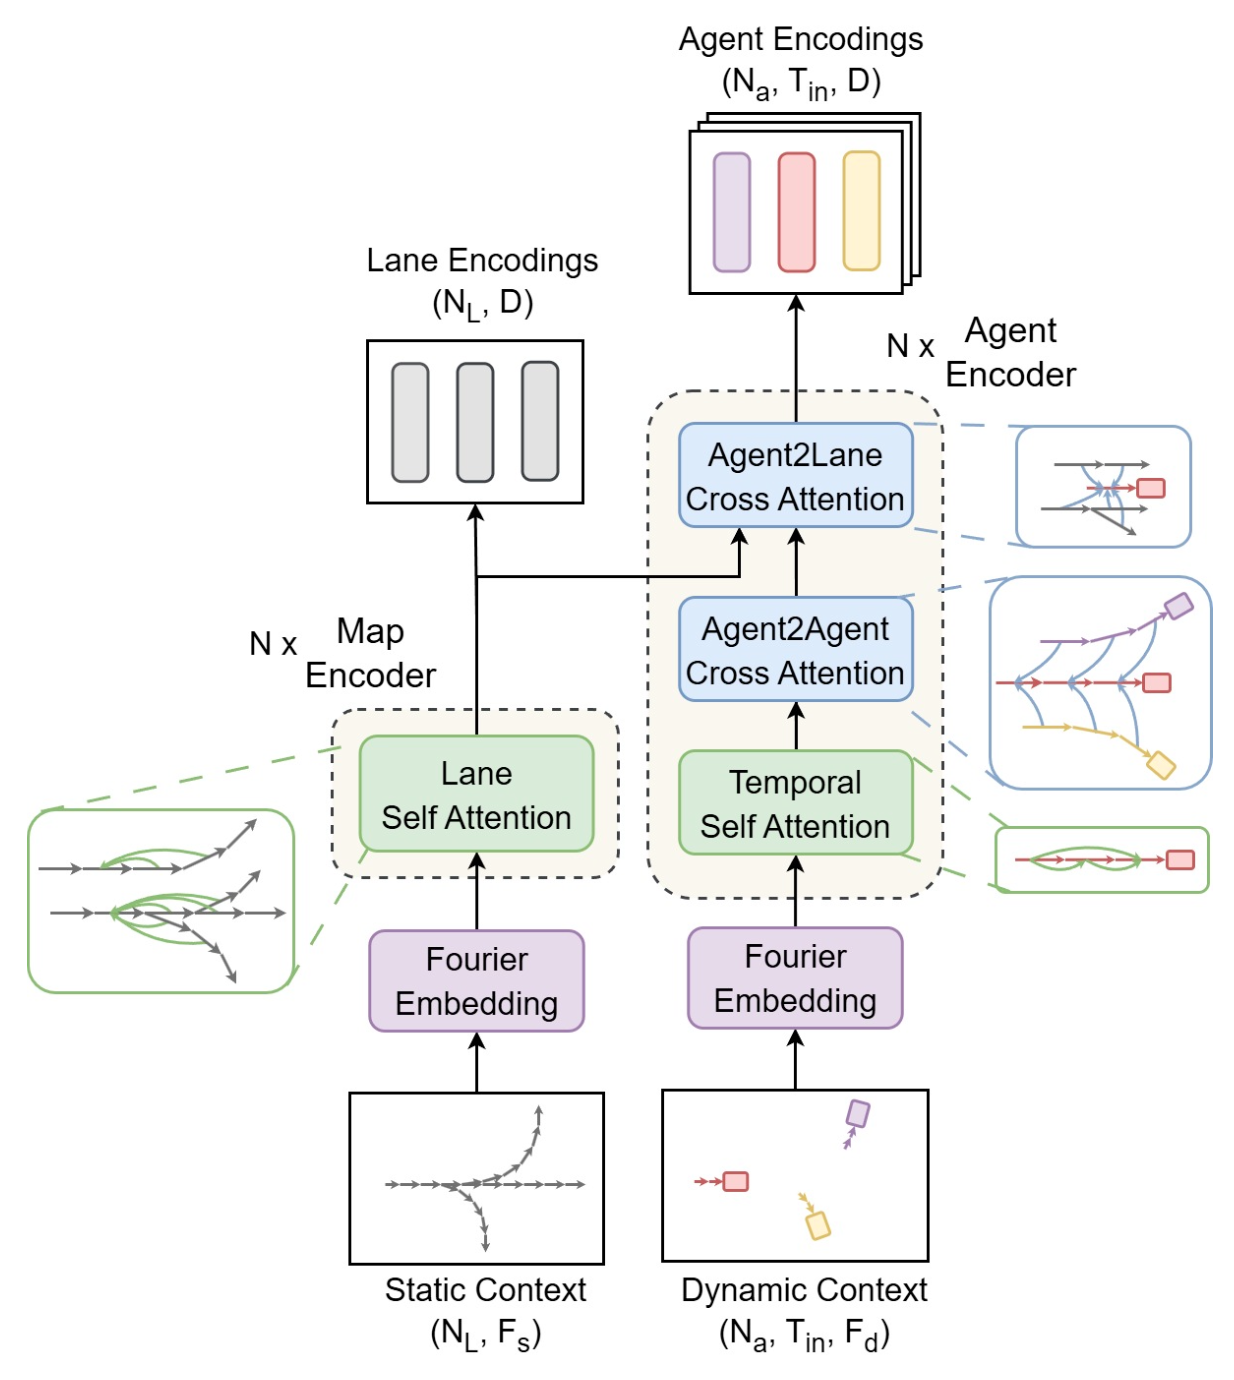
\includegraphics[width=0.7\textwidth]{docs/figures/lmformer_arch_encorder.png}
        \caption{LMFormer encoder: learnable Fourier embeddings, lane self-attention, agent temporal and cross-attentions~\cite{lmformerYadav2025}.}
    \end{figure}
\end{frame}

\begin{frame}{Encoder: Learnable Fourier Embeddings}
    \frametitle{Encoder: Learnable Fourier Embeddings}
    \begin{itemize}
        \item All scalar inputs (lane geometry, motion history) are lifted with \textbf{learnable Fourier features}.
        \item This allows the model to learn spatio-temporal patterns at various, task-adaptive frequencies.
    \end{itemize}
    \begin{equation}
      \label{eq:pres_learnable_fourier_embedding}
    \mathbf{x} \mapsto \text{GeLU}\left(\mathbf{W}_A \begin{bmatrix} \sin(2\pi \mathbf{x} \mathbf{W}_f^T) \oplus \cos(2\pi \mathbf{x} \mathbf{W}_f^T) \end{bmatrix} + \mathbf{B}_\varphi\right) + \mathbf{B}_\psi
    \end{equation}
    \begin{itemize}
        \item[\(\mathbf{W}_f\)] learns which harmonic frequencies to emphasize.
        \item[\(\mathbf{W}_A\)] learns the amplitude of each frequency.
        \item[\(\mathbf{B}_\varphi, \mathbf{B}_\psi\)] are learnable phase shifts and biases.
    \end{itemize}
    \vspace{1em}
    \small{Unlike fixed sinusoidal embeddings, this adapts during training to capture the most informative scales for trajectory prediction.}
\end{frame}

\begin{frame}{Encoder: Attention Mechanisms}
    \frametitle{Encoder: Attention Mechanisms}
    \begin{itemize}
        \item<1-> \textbf{Map (Lane) Encoder:}
              \begin{itemize}
                \item Applies self-attention over lane-segment tokens to capture topology and geometry.
                \item Result: Static scene encodings \(\mathbf{E}_s\).
              \end{itemize}
        \item<2-> \textbf{Agent Encoder:} Stacks three attention modules:
              \begin{enumerate}
                \item Temporal self-attention (agent's own past).
                \item Agent-agent cross-attention (social interactions).
                \item Agent-lane cross-attention (grounding in map).
              \end{enumerate}
              Result: Agent encodings \(\mathbf{E}_d\).
    \end{itemize}
\end{frame}

\begin{frame}{LMFormer: Decoder Architecture}
    \begin{figure}
        \centering
        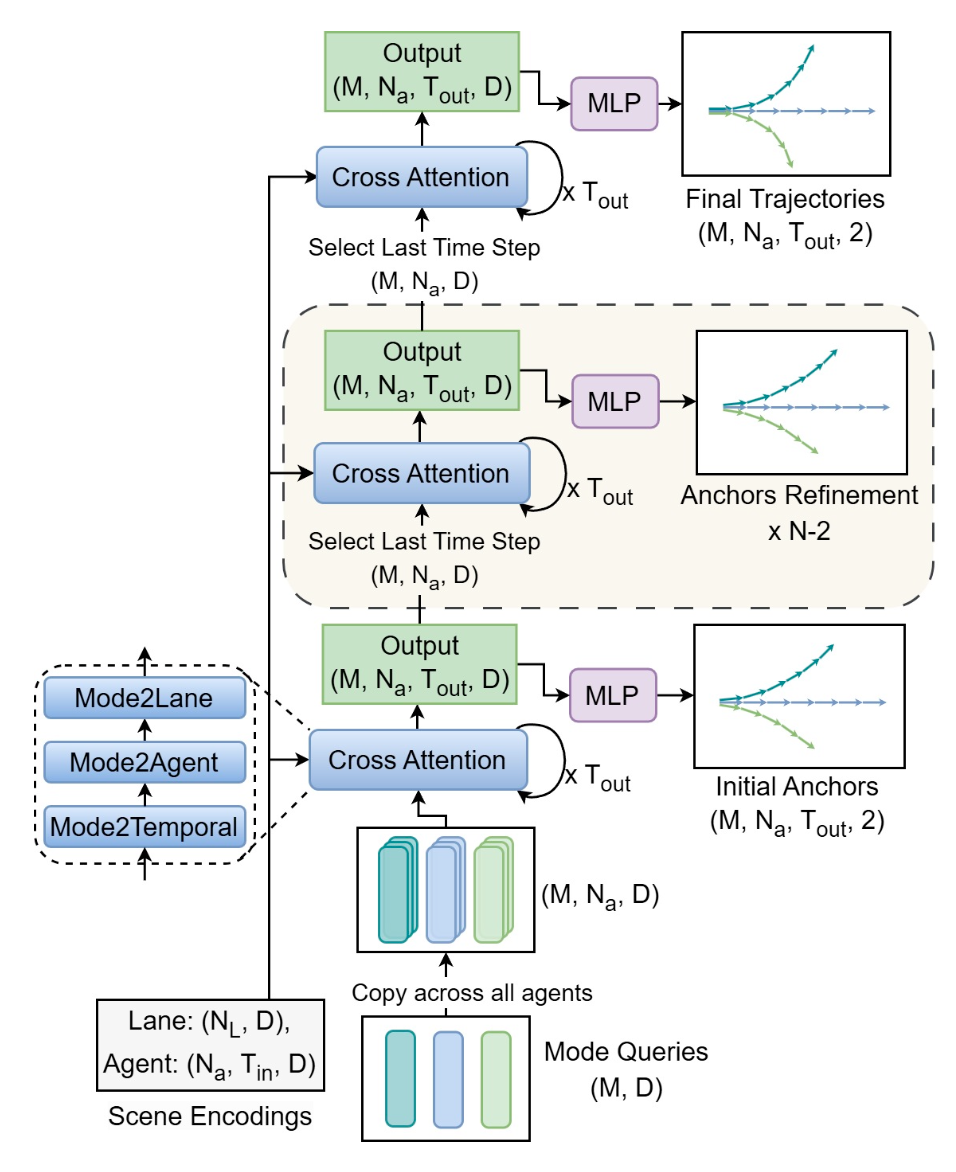
\includegraphics[width=0.7\textwidth]{docs/figures/lmformer_arch_decoder.png}
        \caption{LMFormer decoder: recurrent mode-query cross-attention modules that iteratively generate future motion vectors~\cite{lmformerYadav2025}.}
    \end{figure}
\end{frame}

\begin{frame}[fragile]{Decoder: Recurrent Cross-Attention}
    \frametitle{Decoder: Recurrent Cross-Attention Algorithm}
    \begin{algorithmic}[1]
    \scriptsize
    \Require Agent encodings \(\mathbf{E}_d\), Lane encodings \(\mathbf{E}_s\), Mode anchors \(\mathbf{A}\)
    \Ensure Trajectory sets \(\{\mathcal{T}_{out}^{(i)}\}_{i=1}^{N_{\text{dec}}}\)
    \State \(\mathbf{q} \leftarrow \text{repeat}(\mathbf{A}, N)\) \(\triangleright\) Initialize mode queries
    \For{\(i = 1\) \textbf{to} \(N_{\text{dec}}\)}
        \For{\(t = 1\) \textbf{to} \(T_f\)}
            \State \(\mathbf{q}\leftarrow \text{CrossAttn}(\mathbf{q}, K=V=\mathbf{E}_d[\dots])\) \quad (\textit{Mode2Temporal})
            \State \(\mathbf{q}\leftarrow \text{CrossAttn}(\mathbf{q}, K=V=\mathbf{E}_d[\dots])\) \quad (\textit{Mode2Agent})
            \State \(\mathbf{q}\leftarrow \text{CrossAttn}(\mathbf{q}, K=V=\mathbf{E}_s)\) \quad (\textit{Mode2Lane})
        \EndFor
        \State \(\mathcal{T}_{out}^{(i)} \leftarrow \text{MLP}(\text{updated queries})\)
    \EndFor
    \end{algorithmic}
\end{frame}

\begin{frame}{Decoder: Output and Loss}
    \frametitle{Decoder: Output and Loss}
    \textbf{Output Formulation}
    \begin{itemize}
        \item Every mode query predicts a \textbf{motion-vector chain}:
    \end{itemize}
    \begin{equation}
    \mathcal{T}_{out}^{a,m} = \bigl[(V_1^{a,m},S_1^{a,m}),\dots,(V_{T_f}^{a,m},S_{T_f}^{a,m})\bigr],
    \end{equation}
    where \(V_t\) is a displacement vector and \(S_t\) its uncertainty, parameterizing a Laplacian mixture.

    \vspace{1em}
    \textbf{Loss Formulation}
    \begin{itemize}
        \item Combines winner-takes-all regression loss and classification loss.
        \item Supervises \emph{every} refinement layer to encourage coarse-to-fine refinement.
    \end{itemize}
\end{frame}


\begin{frame}{LMFormer: Qualitative Comparison}
    \frametitle{LMFormer: Qualitative Comparison}
    \begin{columns}[T]
        \begin{column}{0.5\textwidth}
            \textbf{Pros} \greenoplus
            \begin{itemize}
                \item Fully query-centric (\(\mathrm{SE}(2)\) invariant).
                \item Joint multi-agent decoding.
                \item Temporally coherent refinement.
                \item Reduced VRAM vs. QCNet.
            \end{itemize}
        \end{column}
        \begin{column}{0.5\textwidth}
            \textbf{Cons} \redominus
            \begin{itemize}
                \item High VRAM vs. CASPFormer.
                \item Lane-only static context.
                \item Uniform loss weighting.
                \item Generalization challenges.
            \end{itemize}
        \end{column}
    \end{columns}
\end{frame}

\section{Conclusion}

\subsection{A Qualitative Comparison of the Selected Architectures}

\begin{frame}{Relation to CASPNet \& CASPFormer}
    \frametitle{Relation to CASPNet \& CASPFormer}
    \begin{itemize}
        \item \textbf{CASPNet}: Operates on raster grids, predicts per-pixel occupancies.
        \item \textbf{CASPFormer}: Adds deformable attention and vector outputs but remains \emph{agent-centric}.
        \item \textbf{LMFormer}: Discards the raster backbone entirely for a \emph{query-centric} paradigm.
    \end{itemize}
    \vfill
    \begin{alertblock}{Key Trade-off}
    Gains strict symmetry compliance and parallel multi-agent decoding at the cost of a larger key-value cache and higher VRAM demand (\(\approx\)2x CASPFormer).
    \end{alertblock}
\end{frame}


\begin{frame}{Conclusion}
\begin{itemize}
    % TODO: codex bullshit
    \item Scene representation paradigms are crucial for effective trajectory prediction.
    \item Query-centric approaches offer significant advantages in terms of geometric fidelity and computational efficiency.
    \item Future work should focus on optimizing memory usage and exploring hybrid models.
    \item The field is rapidly evolving, with new architectures pushing the boundaries of what is possible in trajectory prediction.
\end{itemize}
\end{frame}

\end{document}

\begin{frame}[allowframebreaks]
  \frametitle{References}
  \bibliographystyle{ieeetr}
  \bibliography{docs/latex/references}
\end{frame}
